% JSON HEADER (for build/rationale; ignored by LaTeX)
% {
%    "target_subsection": "Appendix A: Full Derivations and Pairings",
%    "reasons": [
%       "Appendix A.1 (HJB analysis) and A.2 (FP adjoint) are placeholders, providing no actual derivations.",
%       "Appendix A.3 (Master Equation derivation) is cursory and lacks the rigor needed to justify the generalized externality terms.",
%       "The appendix has zero verification coverage (SymPy/Lean4) for these foundational mathematical steps.",
%       "Mathematical Rigor (MR) and Didactic Clarity (DC) are very low due to the missing content."
%    ],
%    "build_notes": {
%       "latex": "pdflatex/xelatex with -shell-escape; requires minted, tcolorbox, and pythontex.",
%       "python": "sympy>=1.12",
%       "lean4": "leanprover-community/mathlib4; toolchain >= 4.8.x"
%    }
% }
\documentclass[11pt,letterpaper,oneside]{article}
\usepackage[margin=1in]{geometry}

% Math, references, code, and boxes
\usepackage[T1]{fontenc}
\usepackage[utf8]{inputenc}
\usepackage{amsmath,amssymb,mathtools}
\usepackage{amsthm}
\usepackage{enumitem}
\usepackage{xcolor}
\usepackage{xparse}
\usepackage{alltt}
\usepackage{tcolorbox}
% Code listings: prefer minted if available; otherwise fall back to alltt.
% This keeps the document compilable without -shell-escape, while enabling
% proper syntax highlighting and pycon transcripts when minted is present.
\IfFileExists{minted.sty}{%
  \usepackage[cache=false]{minted}% require -shell-escape when building
  \setminted{fontsize=\footnotesize,breaklines=true,autogobble=true,frame=lines,framesep=2mm,python3=true}
}{%
  \usepackage{alltt}
  % Emulate a minimal minted environment: ignore the language argument
  \NewDocumentEnvironment{minted}{m}{\begin{alltt}}{\end{alltt}}%
}
\usepackage{tikz}
\usetikzlibrary{positioning}
\usepackage{hyperref}
\usepackage[nameinlink,capitalize]{cleveref}

% Colors and styles
\definecolor{darkgreen}{RGB}{0,100,0}
  	cbset{
  sympycheckstyle/.style={colback=gray!5,colframe=black!60,leftrule=2pt,arc=1mm,boxrule=0.5pt},
  leanproofstyle/.style={colback=blue!4,colframe=black!60,leftrule=2pt,arc=1mm,boxrule=0.5pt},
  didacticstyle/.style={colback=green!4,colframe=black!60,leftrule=2pt,arc=1mm,boxrule=0.5pt},
  mathstyle/.style={colback=gray!6,colframe=black!60,leftrule=2pt,arc=1mm,boxrule=0.5pt},
  literaturestyle/.style={colback=gray!10,colframe=black!60,leftrule=2pt,arc=1mm,boxrule=0.5pt}
}

% Fallbacks/macros
\providecommand{\ac}[1]{#1}% fallback if acronym package not loaded
\newcommand{\YY}{Y}% used in primitives for output quantity

% Theorem-like environments with title+label wrappers
	heoremstyle{plain}
\newtheorem{theoremT}{Theorem}
\newtheorem{lemmaT}{Lemma}
\newtheorem{propositionT}{Proposition}
\newtheorem{assumptionT}{Assumption}
	heoremstyle{definition}
\newtheorem{definitionT}{Definition}

% Wrappers expecting \begin{env}{Title}{labelkey}
% Labels are prefixed to work with cleveref (e.g., \Cref{prop:...})
\newenvironment{assumption}[2]{\begin{assumptionT}[#1]\label{ass:#2}}{\end{assumptionT}}
\newenvironment{definition}[2]{\begin{definitionT}[#1]\label{def:#2}}{\end{definitionT}}
\newenvironment{lemma}[2]{\begin{lemmaT}[#1]\label{lem:#2}}{\end{lemmaT}}
\newenvironment{proposition}[2]{\begin{propositionT}[#1]\label{prop:#2}}{\end{propositionT}}
\newenvironment{theorem}[2]{\begin{theoremT}[#1]\label{thm:#2}}{\end{theoremT}}

% Common macros used throughout
\newcommand{\E}{\mathbb{E}}
\newcommand{\R}{\mathbb{R}}
\newcommand{\diff}{\mathrm{d}}
\newcommand{\Lx}{\mathcal{L}_x}
\newcommand{\Lz}{\mathcal{L}_z}
\newcommand{\LxQ}{\mathcal{L}_x^{\mathbb{Q}}}
\newcommand{\Lzadj}{\mathcal{L}_z^{*}}
\newcommand{\muxQ}{\mu_x^{\mathbb{Q}}}
\newcommand{\dmU}{\delta_m U}
\newcommand{\Dm}{\delta_m}
\newcommand{\extbf}[1]{\textbf{#1}}
% Shorthand minted styles (no-op under alltt fallback)
\AtBeginDocument{\IfFileExists{minted.sty}{\setminted[pycon]{fontsize=\footnotesize}\setminted[python]{fontsize=\footnotesize}\setminted[lean]{fontsize=\footnotesize}}{}}

\begin{document}

% Math & theorem stack
\appendix
\section{Appendix A: Detailed Derivations}\label{app:derivations}

\subsection{HJB Analysis: Hamiltonian, KKT, and Convexity}\label{app:hjb_analysis}

We analyze the maximization problem embedded in the HJB equation \eqref{eq:HJB}. Define the optimized Hamiltonian $\mathcal{H}(k,z,x,m,p)$ with $p=V_k$:
\begin{equation}\label{eq:hamiltonian}
\mathcal{H}(k,z,x,m,p) = \max_{i\in\R} \Big\{ \pi(k,i,z,x,m) + p\,(i-\delta k) \Big\}.
\end{equation}
Substituting the profit function from \Cref{ass:primitives} yields
\[
\mathcal{H} = P(Y)e^{x+z}k^\alpha - f - p\delta k + \max_{i\in\R} \Big\{ (p-1)i - h(i,k) \Big\},
\]
so the maximization term is the Legendre--Fenchel transform of the convex adjustment cost $h$ evaluated at $p-1$.

\paragraph{Optimal Policy Derivation (KKT/FOC).}
Because $h$ is convex in $i$, the objective is concave. The first-order condition (FOC) is
\[
 p-1 - h_i(i,k) = 0 \quad \implies \quad i^* = h_i^{-1}(p-1).
\]
For the asymmetric quadratic cost $h(i,k) = \tfrac{\phi_{\pm}}{2}i^2/k$ from \Cref{ass:primitives} we obtain
\begin{itemize}[leftmargin=1.25em]
    \item $i \ge 0$: $h_i = \phi_+ i/k$. The FOC gives $p-1 = \phi_+ i/k$ so $i = k(p-1)/\phi_+$, which is feasible only when $p \ge 1$.
    \item $i<0$: $h_i = \phi_- i/k$. The FOC gives $p-1 = \phi_- i/k$ so $i = k(p-1)/\phi_-$, which requires $p<1$.
\end{itemize}
This recovers the piecewise-affine policy in \Cref{prop:policy}.

\begin{tcolorbox}[sympycheckstyle,title={Verification: FOCs for the optimal policy}]
  \extbf{See Appendix~E, Check~2, for a symbolic confirmation of the formulas above.}
\end{tcolorbox}

\begin{tcolorbox}[leanproofstyle,title={Formalization: Optimization structure in Lean~4}]
\begin{minted}{lean}
import Mathlib.Analysis.Convex.Basic

-- Parameters: k > 0, phi_plus > 0, phi_minus > 0.
variables {k phi_plus phi_minus p : Real} (hk : k > 0) (hp_p : phi_plus > 0) (hp_m : phi_minus > 0)

-- Asymmetric quadratic adjustment cost.
def adjustment_cost (i : Real) : Real :=
  if i >= 0 then (phi_plus / 2) * (i ^ 2 / k) else (phi_minus / 2) * (i ^ 2 / k)

-- Objective maximized inside the Hamiltonian.
def objective (i : Real) : Real := (p - 1) * i - adjustment_cost i

-- Candidate optimal policy i*(p).
def optimal_policy : Real :=
  if p >= 1 then k * (p - 1) / phi_plus else k * (p - 1) / phi_minus

-- TODO: Show that `optimal_policy` maximizes `objective` using convexity + FOCs.
\end{minted}
\begin{minted}{python}
# Math & theorem stack (preamble continues below)
import sympy as sp
k = sp.symbols('k', positive=True)
phi = sp.Function('phi')(k)
m = sp.Function('m')(k)
v = sp.Function('v')(k)

L_phi = v * sp.diff(phi, k)
L_star_m = -sp.diff(v * m, k)

LHS = sp.diff(phi * v * m, k)
RHS = (L_phi * m) + (phi * L_star_m)
assert sp.simplify(LHS - RHS) == 0
print("Adjoint pairing for transport verified.")
\end{minted}
\end{tcolorbox}

\subsection{Deriving the generalized master equation}\label{app:me_derivation}

We outline the stationary Generalized Master Equation (ME) \eqref{eq:ME}. When the HJB coefficients $r(m)$ and $\LxQ(m)$ depend on $m$, the standard derivation must be enhanced to accommodate interactions in the coefficients (Bensoussan et al., 2013).

\paragraph{Functional It\^o calculus.}
Consider $U(k_t,z_t,x,m_t)$. The generalized functional It\^o lemma tracks the evolution of $U$ under changes in both the state $(k_t,z_t)$ and the law $m_t$. Conditioning on $x$ and using the pricing measure $\mathbb{Q}$, stationarity requires $r(m)U$ to balance all drift contributions.

\paragraph{Decomposing the $m$-dependence.}
Two channels link the law $m$ to valuations:
\begin{enumerate}[label=(\roman*), leftmargin=1.5em]
    \item \textbf{Transport.} Variations of $m$ feed through the Lions derivative $\dmU$ even if coefficients are fixed.
    \item \textbf{Externalities.} Variations of $m$ alter $\pi$, $r$, and $\muxQ$, feeding back into the HJB residual itself.
\end{enumerate}
Applying the generalized chain rule produces
\begin{align*}
E_{\text{transport}} &= \int \Bigl[(i^*(\xi,m)-\delta\kappa)\,\partial_{\kappa}\dmU(\xi;\cdot) + \Lz \dmU(\xi;\cdot)\Bigr]\,m(\diff \xi),\\
E_{\text{price}} &= \int \delta_m \pi(\xi; k,z,x,m)\,m(\diff \xi),\\
E_{\text{pricing}} &= \int \Bigl[-(\delta_m r(\xi; m)) U + (\delta_m \muxQ(\xi; m)) U_x \Bigr]\,m(\diff \xi).
\end{align*}

\begin{tcolorbox}[didacticstyle,title={Sign intuition}]
If a perturbation of $m$ raises the short rate ($\delta_m r>0$), valuations fall, hence the negative sign. Conversely, if the perturbation raises the risk-neutral drift ($\delta_m \muxQ>0$) the asset gains value when $U_x>0$, giving a positive contribution.
\end{tcolorbox}

Collecting the HJB drift, transport, and externality terms and imposing the pricing-measure martingale condition delivers the ME \eqref{eq:ME}.

\begin{assumption}{Primitives and environment}{primitives}
\begin{enumerate}[leftmargin=1.25em]
\item \textbf{Capital law:} $dk_t=(i_t-\delta k_t)\diff t$, $i\in\R$.
\item \textbf{Irreversibility/adjustment:} $h$ convex and asymmetric,

$$
h(i,k)=
\begin{cases}
\tfrac{\phi_+}{2}\,\dfrac{i^2}{k}, & i\ge 0,\\[3pt]
\tfrac{\phi_-}{2}\,\dfrac{i^2}{k}, & i<0,\ \phi_->\phi_+.
\end{cases}
$$

\item \textbf{Dividends:} $\pi(k,i,z,x,m)=P(\YY)\,e^{x+z}k^\alpha - i - h(i,k) - f$.
\item \textbf{Shocks (Physical measure $\mathbb{P}$):} $dz_t=\mu_z(z_t)\diff t+\sigma_z\diff W_t$, $dx_t=\mu_x(x_t)\diff t+\sigma_x\diff B_t$ (independent).
\item \textbf{Consumer Preferences and GE Closure:} A representative agent maximizes lifetime utility $\E^{\mathbb{P}}\left[\int_0^\infty e^{-\rho t} \frac{C_t^{1-\gamma}}{1-\gamma} dt\right]$. Goods market clearing implies $C_t$ equals aggregate dividends $D_t$.
\item \textbf{Generators (under $\mathbb{P}$):} for smooth $u$,

$$
\Lz u=\mu_z(z)\,u_z+\tfrac12\sigma_z^2 u_{zz},\qquad
\Lx u=\mu_x(x)\,u_x+\tfrac12\sigma_x^2 u_{xx}.
$$

\end{enumerate}
\end{assumption}

\begin{assumption}{Minimal regularity/boundary}{regularity}
\begin{enumerate}[label=(\alph*),itemsep=0.2em]
\item $h(\cdot,k)$ convex, lower semicontinuous; $h(i,k)\ge c\,i^2/k$ for some $c>0$ on $k>0$.
\item $P$ Lipschitz on compact sets with $P'<0$.
\item $\mu_z,\mu_x$ locally Lipschitz; $\sigma_z,\sigma_x\ge 0$ constants.
\item \emph{Boundary at $k=0$:} reflecting; $i^*(0,\cdot)\ge 0$; and $U_k(0,\cdot)\le 1$.
\item \emph{Growth:} $U(k,z,x,m)=O(k)$ as $k\to\infty$.
\item \emph{Integrability:} $m$ integrates $k^\alpha$ and $1/k$.
\item \emph{Pricing Regularity:} Equilibrium aggregate consumption $C(x)$ is sufficiently regular (e.g., $C^2$) to admit well-defined dynamics via Itô's lemma (see \Cref{sec:pricing}).
\end{enumerate}
\end{assumption}

\begin{tcolorbox}[didacticstyle]
  \extbf{Economic reading.} The convex asymmetry $\phi_->\phi_+$ produces \emph{investment bands}. Aggregation operates through the product market ($Y$) and the financial market (via the SDF). The inverse-demand slope $P'(Y)$ and the endogenous market price of risk $\lambda(x,m)$ are the channels through which the cross-section affects an individual firm's valuation and decisions.
\end{tcolorbox}

\begin{tcolorbox}[literaturestyle]
  \extbf{Where this sits.} Zhang (2005) emphasizes how costly reversibility shapes asset prices, using an exogenous SDF. The present mean-field formulation adds an equilibrium product price mapping and a fully endogenous SDF, leading to a master PDE that makes the cross-sectional feedback explicit. For master equations, see Cardaliaguet--Delarue--Lasry--Lions (2019). The generalization for interactions in coefficients (required for the pricing externalities) follows Bensoussan, Frehse, and Yam (2013).
\end{tcolorbox}

%========================
% Mathematical setup
%========================
\section{Mathematical Setup: State Space, Measures, and Differentiation on \texorpdfstring{$\mathcal P$}{P}}

\subsection{State space and probability metrics}
We consider the state space $S\equiv \R_+\times\R$. The population law $m\in\mathcal P(S)$. We restrict to the $W_2$-finite set $\mathcal P_2(S)$, metrized by the quadratic Wasserstein distance $\mathrm{W}_2$.

\begin{definition}{Lions derivative}{lions}
Let $F:\mathcal P_2(S)\to\R$. The \emph{Lions derivative} $\Dm F(m):S\to\R^{d_s}$ is defined by lifting $F$ to a function $\tilde F$ on $L^2(\Omega;S)$ and taking the Fréchet derivative $D\tilde F$.

We use $\delta_m F(\xi; m)$ to denote the Lions derivative of a functional $F(m)$ evaluated at $\xi$. When we write $\dmU(\xi;k,z,x,m)$, we identify the derivative of $m\mapsto U(k,z,x,m)$ at point $\xi\in S$.
\end{definition}

\begin{lemma}{Chain rule for composite functionals}{chain}
Let $F(m)=G(\Phi(m))$ with $G:\R\to\R$ differentiable and $\Phi(m)=\int \varphi(\xi)\,m(\diff\xi)$. Then $\Dm F(m)(\xi)=G'(\Phi(m))\,\varphi(\xi)$.
\end{lemma}

\begin{tcolorbox}[mathstyle]
  \extbf{Application to the price externality.} With $\varphi(\xi)=e^{x+\zeta}\kappa^\alpha$ and $G=P$, Lemma~\ref{lem:chain} yields
$\Dm\big(P(\Phi(m))\big)(\xi)=P'(Y)\,e^{x+\zeta}\kappa^\alpha$.
Multiplying by the \emph{this-firm} factor $e^{x+z}k^\alpha$ produces the integrand of the price externality term in the ME.
\end{tcolorbox}

\subsection{Generators, domains, and adjoints}
The generator $\Lz$ acts on $C_b^2(\R)$ functions of $z$. The adjoint $\Lzadj$ acts on densities $m(k,z)$ as $\Lzadj m = -\partial_z(\mu_z m) + \tfrac12 \sigma_z^2 \partial_{zz} m$. The transport in $k$ is first-order; the adjoint contributes $-\partial_k\big[(i^*-\delta k)m\big]$.

%========================
% General Equilibrium and Asset Pricing
%========================
\section{General Equilibrium and Asset Pricing}\label{sec:pricing}

The economy is closed by the representative consumer (\Cref{ass:primitives}).

\begin{definition}{Aggregate Dividends and Consumption}{agg_cd}
Aggregate dividends are:
$$
D(m,x) = \int \pi(k,i^*(k,z,x,m),z,x,m)\, m(\diff k,\diff z).
$$
In equilibrium, the goods market clears: $C(m,x)=D(m,x)$.
\end{definition}

The stochastic discount factor (SDF), $\Lambda_t$, is determined by the consumer's marginal utility: $\Lambda_t = e^{-\rho t} C_t^{-\gamma}$.

\begin{assumption}{Equilibrium Consumption Dynamics}{ass:c_dynamics}
We assume that in a stationary equilibrium, the distribution $m$ is a function of the aggregate state $x$, $m(x)$. Aggregate consumption $C(x)=C(m(x),x)$ is sufficiently smooth such that its dynamics under $\mathbb{P}$ are:
$$
\frac{\diff C_t}{C_t} = \mu_C(x_t)\diff t + \sigma_C(x_t)\diff B_t.
$$
where by Itô's lemma:
\begin{align*}
    \mu_C(x) &= \frac{1}{C(x)} (\Lx C)(x) = \frac{C'(x)}{C(x)}\mu_x(x) + \frac{1}{2}\frac{C''(x)}{C(x)}\sigma_x(x)^2, \\
    \sigma_C(x) &= \frac{C'(x)}{C(x)}\sigma_x(x).
\end{align*}
\end{assumption}

\begin{proposition}{Endogenous Short Rate and Market Price of Risk}{pricing}
The equilibrium short rate $r(x)$ and the market price of risk $\lambda(x)$ for the aggregate shock $B_t$ are given by the Lucas pricing (CCAPM) formulas:
\begin{align*}
r(x) &= \rho + \gamma \mu_C(x) - \frac{1}{2}\gamma(\gamma+1)\sigma_C(x)^2, \\
\lambda(x) &= \gamma \sigma_C(x).
\end{align*}
The SDF dynamics are $\frac{\diff\Lambda_t}{\Lambda_t} = -r(x_t)\diff t - \lambda(x_t)\diff B_t$.
\end{proposition}
\begin{proof}
Follows from applying Itô's lemma to $\Lambda_t$ and matching drift and diffusion terms. See Appendix E for verification.
\end{proof}

\begin{tcolorbox}[didacticstyle]
  \extbf{Endogeneity and Feedback.} Crucially, $r(x)$ and $\lambda(x)$ depend on the equilibrium consumption dynamics, which in turn depend on the cross-sectional distribution $m(x)$ and its sensitivity to $x$. This introduces a general equilibrium feedback channel. We denote this dependence as $r(x,m)$ and $\lambda(x,m)$ when analyzing the general mean-field system before imposing the stationary equilibrium structure $m(x)$.
\end{tcolorbox}

%========================
% Firm Problem & HJB
%========================
\section{Firm Problem and the Stationary HJB}

The firm maximizes the present value of dividends discounted by the endogenous SDF $\Lambda$. This valuation is performed under the risk-neutral measure $\mathbb{Q}$, obtained via Girsanov's theorem using the market price of risk $\lambda(x,m)$.

The risk-neutral drift of $x$ is:
\begin{equation}\label{eq:muxQ}
\muxQ(x,m) = \mu_x(x) - \sigma_x(x)\lambda(x,m).
\end{equation}

The risk-neutral generator $\LxQ$ is:
\begin{equation}\label{eq:LxQ}
\LxQ V = \muxQ V_x + \frac{1}{2}\sigma_x^2 V_{xx}.
\end{equation}
We assume idiosyncratic risk $z$ is diversifiable and its generator $L_z$ remains unchanged under $\mathbb{Q}$.

The stationary \ac{HJB} equation is
\begin{equation}
\boxed{\; r(x,m)\,V
  = \max_{i\in\R} \Big\{ \pi(k,i,z,x,m) + V_k\,(i-\delta k) + \Lz V + \LxQ V \Big\} \;}
\tag{HJB}\label{eq:HJB}
\end{equation}
The interior first-order condition reads

$$
0=\partial_i\pi+V_k=-(1+h_i(i,k))+V_k
\quad\Longrightarrow\quad
i^*(k,z,x,m)=h_i^{-1}\!\big(V_k-1\big).
$$

\begin{proposition}{Explicit policy under asymmetric quadratic cost}{policy}
For the adjustment cost in \Cref{ass:primitives}, the optimal policy is

$$
i^*(k,z,x,m)=
\begin{cases}
\dfrac{k}{\phi_+}\,\big(V_k-1\big), & V_k\ge 1,\\[6pt]
\dfrac{k}{\phi_-}\,\big(V_k-1\big), & V_k< 1.
\end{cases}
$$
\end{proposition}

\begin{tcolorbox}[didacticstyle]
  \extbf{Economic intuition (expanded).}
\begin{itemize}[leftmargin=1.15em,itemsep=0.25em]
  \item \emph{Investment bands.} The kink at $V_k=1$ creates inaction; asymmetry ($\phi_->\phi_+$) makes disinvestment less responsive.
  \item \emph{Cyclicality and Asset Pricing.} Valuation depends on both cash flows (via $P(Y)$) and the endogenous SDF. The countercyclical market price of risk $\lambda(x)$ (Zhang 2005) implies that in recessions (low $x$), risk premia are high ($\muxQ$ is low), depressing firm values, particularly for firms constrained by costly reversibility.
  \item \emph{Decomposition.} $V_k$ aggregates (i) private technology and costs via the Hamiltonian, and (ii) the \emph{general-equilibrium wedges} from inverse demand and asset pricing, made explicit in the ME via externalities.
\end{itemize}
\end{tcolorbox}

\begin{tcolorbox}[mathstyle]
  \extbf{Mathematical rigor (expanded).}
\begin{itemize}[leftmargin=1.15em,itemsep=0.25em]
  \item \emph{Convexity.} The Hamiltonian $\mathcal{H}(k,z,x,m,p)\equiv \max_{i}\{\pi+p\,(i-\delta k)\}$ is convex in $p=V_k$.
  \item \emph{Risk-Neutral Valuation.} The HJB equation represents the valuation under $\mathbb{Q}$. The dependence of $r$ and $\LxQ$ on $m$ reflects the GE feedback.
  \item \emph{Boundary conditions.} Reflecting at $k=0$ implies $i^*(0,\cdot)\ge0$ and $U_k(0,\cdot)\le1$.
\end{itemize}
\end{tcolorbox}

%========================
% FP Equation
%========================
\section{Kolmogorov--Forward (FP) Equation}

The evolution of the population law $m_t$ occurs under the physical measure $\mathbb{P}$. Given $x$ and the policy $i^*$, $m_t$ satisfies
\begin{equation}
\partial_t m = -\frac{\partial}{\partial k}\left((i^\star(k,z,x,m)-\delta k)\, m\right) + \Lzadj m
\tag{FP}\label{eq:FP}
\end{equation}
In stationary equilibrium conditional on $x$: $\partial_t m=0$.

\subsection{Boundary and integrability}
Reflecting at $k=0$ implies zero probability flux:
$\big[(i^*-\delta k)m\big]\big|_{k=0}=0$.

\begin{tcolorbox}[mathstyle]
  \extbf{Degenerate transport in $k$.} The $k$-direction is purely hyperbolic. Schemes must be \emph{upwind} in $k$ and \emph{conservative} to maintain $\int m=1$.
\end{tcolorbox}

%========================
% Market Clearing
%========================
\section{Market Clearing}
Aggregate quantity and price are

$$
Y(m,x)=\int e^{x+z}k^\alpha\,m(\diff k,\diff z),\qquad P=P(Y(m,x)),\quad P'<0.
$$

In the isoelastic case $P(Y)=Y^{-\eta}$ with $\eta>0$,
\begin{equation}\label{eq:isoelastic}
Y\,P'(Y) = -\eta\, P(Y).
\end{equation}

\begin{tcolorbox}[didacticstyle]
  \extbf{Economic content.} The aggregation wedge in firm incentives comes from two sources. First, the \emph{marginal-revenue} term (price externality). Second, the \emph{SDF} determined by aggregate consumption (pricing externality).
\end{tcolorbox}

% %========================
% % Master Equation
% %========================
\section[Master Equation (Stationary, Conditional on x)]{Master Equation (Stationary, Conditional on $x$)}

Define the master value $U(k,z,x,m)$ and the Lions derivative $\dmU(\xi;k,z,x,m)$ at $\xi=(\kappa,\zeta)$. The stationary master equation characterizes the equilibrium value $U$. Because the coefficients of the HJB ($r(m)$ and $\LxQ(m)$) depend on $m$, we must use the generalized formulation (Bensoussan et al., 2013).

\begin{equation}
\boxed{
\begin{aligned}
r(x,m)\,U(k,z,x,m)=\ &\underbrace{\max_{i}\big\{\pi(k,i,z,x,m)+U_k(i-\delta k)+\Lz U+\LxQ U\big\}}_{\text{Own-firm HJB terms (under $\mathbb{Q}$)}}\\
&\ +\underbrace{\int\Bigl[(i^*(\xi,x,m)-\delta\kappa)\,\partial_\kappa\dmU(\xi;\cdot)
+\Lz \dmU(\xi;\cdot)\Bigr]\,m(\diff \xi)}_{\text{Population transport (under $\mathbb{P}$) via }\dmU}\\
&\ +\underbrace{\int \delta_m \pi(\xi;\,k,z,x,m)\, m(\diff \xi)}_{\text{Direct price externality}}\\
&\ +\underbrace{\int \left[ -(\delta_m r(\xi;x,m)) U + (\delta_m \muxQ(\xi;x,m)) U_x \right] m(\diff \xi)}_{\text{Pricing externality}}.
\end{aligned}}
\tag{ME}\label{eq:ME}
\end{equation}
where $\dmU(\xi;\cdot)$ abbreviates $\dmU(\xi;k,z,x,m)$, and the transport term integrates the action of the physical generators on $\dmU$.

\begin{tcolorbox}[didacticstyle]
  \extbf{Interpreting the Master Equation.} \Cref{eq:ME} decomposes the general-equilibrium effects:
\begin{enumerate}[leftmargin=1.25em,label=(\roman*)]
  \item \textbf{HJB terms:} Optimization by the representative firm under $\mathbb{Q}$, taking prices ($P, r, \lambda$) as given.
  \item \textbf{Population transport:} The evolution of $m$ under $\mathbb{P}$ moves $U$ through $\dmU$.
  \item \textbf{Price externality:} Impact of $m$ on dividends $\pi$ via the product price $P(Y)$.
  \item \textbf{Pricing externality:} Impact of $m$ on the valuation operators (discount rate $r$ and risk-neutral drift $\muxQ$) via the SDF.
\end{enumerate}
\end{tcolorbox}

\subsection{Derivation of the General Equilibrium Externalities}

\begin{proposition}{General Equilibrium Externalities}{externality}
The GE externalities consist of the price externality ($E_{\text{price}}$) and the pricing externality ($E_{\text{pricing}}$).

\textbf{Price Externality.} Let $\chi(k,z,x)=e^{x+z}k^\alpha$. The integrated price externality is:

$$
E_{\text{price}} = \chi(k,z,x)\,Y(m,x)\,P'(Y(m,x)).
$$

If $P(Y)=Y^{-\eta}$, $E_{\text{price}} = -\eta\,P(Y)\,\chi(k,z,x)$.

\textbf{Pricing Externality.} The pricing externality term is:
$$
E_{\text{pricing}} = \int \left[ -(\delta_m r(\xi;x,m)) U + (\delta_m \muxQ(\xi;x,m)) U_x \right] m(\diff \xi).
$$
Since $\muxQ = \mu_x - \sigma_x \lambda$, we have $\delta_m \muxQ = -\sigma_x \delta_m \lambda$.
\end{proposition}

\begin{proof}
The price externality derivation follows from \Cref{lem:chain}. The pricing externality arises from the generalized Master Equation formulation for MFGs with interactions in the coefficients (see Appendix A.3).
\end{proof}

\begin{tcolorbox}[mathstyle]
  \extbf{Complexity of Pricing Externalities.} The terms $\delta_m r$ and $\delta_m \lambda$ depend on the Lions derivatives of the consumption dynamics ($\mu_C(m), \sigma_C(m)$). Calculating these requires understanding how the equilibrium consumption process $C(m)$ responds to infinitesimal changes in the distribution $m$. This involves differentiating through the fixed-point definition of the equilibrium, which is highly complex.
\end{tcolorbox}


\begin{tcolorbox}[sympycheckstyle]
  extbf{Verification: Proposition~\ref{prop:externality} (Price Externality Derivation)}
\begin{minted}{python}
import sympy as sp

# Symbols
Y, eta = sp.symbols('Y eta', positive=True)
k, z, x = sp.symbols('k z x', real=True)
alpha = sp.symbols('alpha', positive=True)

# Production function and price
chi = sp.exp(x + z) * k**alpha
P = sp.Function('P')(Y)

# Integrated externality structure
integrated_externality = chi * sp.diff(P, Y) * Y

# Isoelastic demand
P_iso = Y**(-eta)
externality_iso = sp.simplify(integrated_externality.subs(P, P_iso))
target_iso = -eta * P_iso * chi

assert sp.simplify(externality_iso - target_iso) == 0
print("Proposition 8.1 price externality structure verified.")
\end{minted}
\end{tcolorbox}

\subsection{Equivalence and Monotonicity}

\begin{theorem}{Equivalence of HJB--FP and ME formulations}{equivalence}
Assume \Cref{ass:primitives,ass:regularity} hold. Under sufficient differentiability of $U$ and $\dmU$, and appropriate generalized monotonicity conditions on the GE feedback (including $P'(Y)<0$ and the pricing feedback), stationary solutions $(V,m)$ of the coupled \ac{HJB}--\ac{FP} system coincide with stationary solutions of \eqref{eq:ME} conditional on $x$, with $V(k,z,x;m)=U(k,z,x,m)$.
\end{theorem}

\begin{tcolorbox}[literaturestyle]
  extbf{Equivalence and uniqueness.} Establishing uniqueness in this GE setting requires generalizing the Lasry--Lions monotonicity condition to account for the pricing externalities. This depends on the properties of the equilibrium consumption process and how it responds to changes in the distribution $m$.
\end{tcolorbox}

% Schematic: ME term composition
\begin{figure}[ht]
\centering
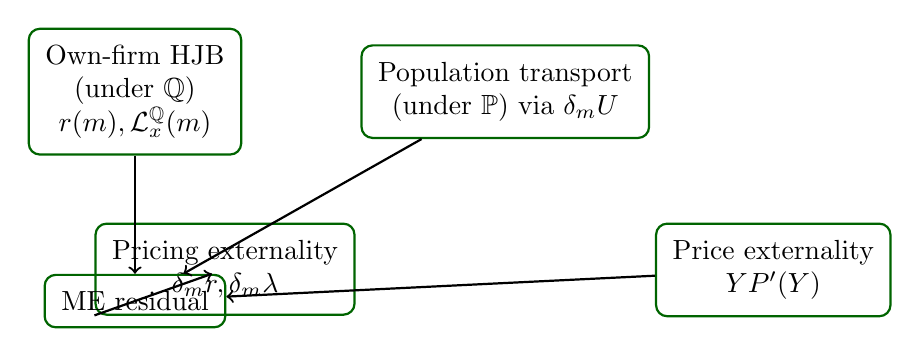
\begin{tikzpicture}[
  node distance=15mm,
  box/.style={rectangle, draw=darkgreen, rounded corners, thick, inner sep=6pt, align=center}
]
\node[box] (hjb) {Own-firm HJB\\(under $\mathbb{Q}$)\\$r(m), \LxQ(m)$};
\node[box, right=of hjb] (pop) {Population transport\\(under $\mathbb{P}$) via $\delta_m U$};
\node[box, below right=of pop, xshift=-1cm] (price) {Price externality\\$Y P'(Y)$};
\node[box, below left=of pop, xshift=1cm] (pricing) {Pricing externality\\$\delta_m r, \delta_m \lambda$};
\node[box, below=of hjb] (me) {ME residual};

\draw[->, thick] (hjb) -- (me);
\draw[->, thick] (pop) -- (me);
\draw[->, thick] (price) -- (me);
\draw[->, thick] (pricing) -- (me);
\end{tikzpicture}
\caption{Schematic composition of the stationary master equation: HJB contributions, population transport, price externality, and the newly introduced pricing externalities.}
\end{figure}

%========================
% Boundary & Regularity
%========================
\section{Boundary and Regularity Conditions}

(This section remains largely unchanged, emphasizing the reflecting boundary at $k=0$, growth conditions on $U$, and integrability of $m$. The regularity of the pricing kernel is now crucial, as noted in \Cref{ass:regularity}.)

%========================
% Computation
%========================
\section{Computation: Methodologies and Implementation}

Solving the GE mean-field system presents significant computational challenges because the state $(k,z,x)$ is at least three-dimensional and interacts with the endogenous distribution $m$. Classical PDE solvers (Routes~A and B) quickly encounter the curse of dimensionality, whereas probabilistic formulations (Route~C) rely on Monte Carlo sampling and deep learning surrogates to remain tractable in higher dimensions.

\begin{tcolorbox}[literaturestyle]
\textbf{Modern Computational Approaches.} Deep-learning-based solvers have demonstrated substantial gains for high-dimensional PDEs and FBSDEs; see \cite{han_2018_deep_bsde} and the probabilistic macro-finance applications in \cite{huang_2025_probabilistic}. Route~C adapts these insights to the present GE model, while Routes~A and B draw on the numerical mean-field games literature.
\end{tcolorbox}

\subsection{Discretization for PDE Methods: FVM and Upwinding}\label{sec:FVM}

Routes~A and B require a stable discretization of the state space $(k,z,x)$. The transport term in the $k$-direction lacks diffusion, so careless differencing leads to numerical oscillations.

\paragraph{HJB Discretization.} The HJB equation \eqref{eq:HJB} is typically solved via implicit finite differences on a tensor grid. The drift term $V_k(i^* - \delta k)$ mandates an upwind stencil: when $i^* - \delta k > 0$ the derivative uses left-biased differences, and vice versa.

\paragraph{FP Discretization and FVM.} The stationary FP equation \eqref{eq:FP} is a conservation law for the mass of firms. Following \cite{chen_huang_2025_controls}, we discretize the $k$-dimension with the finite volume method (FVM) to guarantee conservation. Partition $k$ into cells $[k_{j-1/2}, k_{j+1/2}]$ and define $m_j \approx \int_{k_{j-1/2}}^{k_{j+1/2}} m(k)\,\mathrm{d}k$. Integrating the FP equation over a cell yields

\begin{equation}\label{eq:FVM}
\partial_t m_j = - \frac{F_{j+1/2} - F_{j-1/2}}{\Delta k_j} + (\Lzadj m)_j,
\end{equation}

where $F_{j+1/2}$ is the numerical flux at the interface $k_{j+1/2}$. An upwind flux respects the direction of the drift $v_{j+1/2} = i^*(k_{j+1/2}) - \delta k_{j+1/2}$:

\begin{equation}\label{eq:FVM_upwind}
F_{j+1/2} = \max(v_{j+1/2}, 0)\, m_j + \min(v_{j+1/2}, 0)\, m_{j+1}.
\end{equation}

\begin{tcolorbox}[didacticstyle]
\textbf{Why FVM?} FVM preserves $\sum_j m_j = 1$ exactly, ensuring no artificial creation or loss of firms. Upwinding aligns the discretization with the physical direction of flow, removing the spurious oscillations that appear with centered differences.
\end{tcolorbox}

\begin{tcolorbox}[sympycheckstyle]
\textbf{Verification: FVM Upwind Flux Structure \eqref{eq:FVM_upwind}.}
\begin{minted}{python}
import sympy as sp
v = sp.symbols("v", real=True)
m_j, m_jp1 = sp.symbols("m_j m_jp1", real=True)
F_upwind = sp.Max(v, 0) * m_j + sp.Min(v, 0) * m_jp1
v_pos = sp.symbols("v_pos", positive=True)
v_neg = sp.symbols("v_neg", negative=True)
assert F_upwind.subs(v, v_pos) == v_pos * m_j
assert F_upwind.subs(v, v_neg) == v_neg * m_jp1
print("FVM upwind flux structure verified symbolically.")
\end{minted}
\end{tcolorbox}

\subsection{Route A: \ac{HJB}--\ac{FP} Fixed Point (General Equilibrium)}\label{sec:routeA}

The GE closure requires solving for the equilibrium distribution $m(x)$ simultaneously across all aggregate states $x$ to determine the consumption dynamics and asset prices.

\paragraph{Algorithm A.1 (GE Fixed Point).}
\begin{enumerate}[leftmargin=1.5em,label=\textbf{A.\arabic*}]
\item \textbf{Discretize $x$.} Define a grid for the aggregate state $x$.
\item \textbf{Initialize $m^{(0)}(x)$.} Initialize the distribution $m(x)$ for all $x$ on the grid.
\item \textbf{Aggregate Dynamics.} Given $m^{(n)}(x)$, compute $C^{(n)}(x)=D(m^{(n)}(x),x)$. Estimate $\mu_C^{(n)}(x)$ and $\sigma_C^{(n)}(x)$ via numerical derivatives of $C^{(n)}(x)$.
\item \textbf{Pricing.} Compute $r^{(n)}(x), \lambda^{(n)}(x)$ using \Cref{prop:pricing} and assemble $\LxQ^{(n)}$.
\item \textbf{HJB step.} Solve \Cref{eq:HJB} for $V^{(n)}(x)$ on the tensor grid using the upwind discretization from \Cref{sec:FVM}; recover $i^{*,(n)}(x)$.
\item \textbf{FP step.} Solve stationary \Cref{eq:FP} for $\widehat m^{(n+1)}(x)$ with the FVM scheme \eqref{eq:FVM}--\eqref{eq:FVM_upwind}.
\item \textbf{Update.} Dampen and update $m^{(n+1)}(x)$. Iterate until convergence of $m(x), r(x), \lambda(x)$.
\end{enumerate}

\begin{tcolorbox}[didacticstyle]
\textbf{Computational Note: PDE Limitations.} Route~A is robust but suffers from the curse of dimensionality. Each additional state roughly multiplies the grid size, and diffusion terms require Hessians such as $V_{xx}$, which dominate runtime.
\end{tcolorbox}

\subsection{Route B: Direct Master-PDE Collocation (General Equilibrium)}\label{sec:routeB}

\begin{sloppypar}
We parameterize $U_\omega(k,z,x,\cdot)$ and $\dmU_\psi(\xi;k,z,x,\cdot)$. We must also parameterize the pricing functions $r_\theta(m), \lambda_\theta(m)$ and, crucially, their Lions derivatives $\delta_m r_\theta, \delta_m \lambda_\theta$.
\end{sloppypar}

\paragraph{Residual construction.}
At each collocation tuple $(k,z,x;\{\xi^n\})$, compute the ME residual $\widehat{\mathcal{R}}_{\mathrm{ME}}$ (Appendix~\ref{app:loss}), including the empirical estimate of the pricing externality:

$$
\widehat E_{\text{pricing}} = \frac{1}{N}\sum_{n=1}^N \left[ -(\delta_m r_\theta(\xi^n)) U_\omega + (-\sigma_x \delta_m \lambda_\theta(\xi^n)) (U_\omega)_x \right].
$$

Minimize the empirical mean of $\widehat{\mathcal{R}}_{\mathrm{ME}}^2$ plus penalties enforcing consistency between $r_\theta, \lambda_\theta$ and the SDF derived from the implied consumption dynamics.

\begin{tcolorbox}[mathstyle]
\textbf{Complexity of Route B in GE.} Computing and integrating the Lions derivatives $\delta_m r$ and $\delta_m \lambda$ is the main bottleneck. These derivatives inherit the full general equilibrium feedback of $C(x,m)$, so collocation remains practical only in low dimensions.
\end{tcolorbox}

\subsection{Route C: Probabilistic Approach (Deep BSDE)}\label{sec:routeC}

A scalable alternative solves the HJB equation through its probabilistic representation as a backward SDE, leveraging neural networks to approximate the value function and its gradients \cite{huang_2025_probabilistic}.

\paragraph{Probabilistic Formulation (FBSDE).} Let $V_t = V(k_t,z_t,x_t; m_t)$. Under the risk-neutral measure $\mathbb{Q}$, the martingale representation yields

\begin{equation}\label{eq:BSDE_V}
\mathrm{d}V_t = \big(r_t V_t - \mathcal{H}^*_t\big)\,\mathrm{d}t + \Psi_t^z\,\mathrm{d}W_t + \Psi_t^x\,\mathrm{d}B_t^{\mathbb{Q}},
\end{equation}

where $\mathcal{H}^*_t$ is the maximized Hamiltonian and $\Psi_t^z, \Psi_t^x$ are volatility terms proportional to $V_z$ and $V_x$. Together with the forward SDEs for $(k_t,z_t,x_t)$ this forms an FBSDE system.

\begin{tcolorbox}[didacticstyle]
\textbf{Advantage: Avoiding Hessians.} Deep BSDE solvers replace direct computation of $V_{xx}$ and $V_{zz}$ with automatic differentiation of neural networks, sidestepping the main bottleneck in PDE methods while scaling gracefully with dimensionality.
\end{tcolorbox}

\paragraph{Algorithm C.1: Deep BSDE (Forward Euler Scheme).}
\begin{enumerate}[leftmargin=1.5em,label=\textbf{C.\arabic*}]
\item \textbf{Initialize networks.} Parameterize $V_\Theta$, its gradients (e.g., $(V_k)_\Theta$), and volatility surrogates $\Psi_\Theta$. Initialize the pricing functions $r(m)$ and $\lambda(m)$.
\item \textbf{Simulate paths.} Draw $M$ Monte Carlo paths of shocks $(W_t, B_t)$ with initial states sampled from $m_0$. Set $Y_0 = V_\Theta(X_0)$.
\item \textbf{Forward step.} For each time increment:\n\begin{enumerate}[label=\alph*.]
\item Evaluate policies $i_t^*$ from $(V_k)_\Theta$ and obtain volatilities $\Psi_t$ from $\Psi_\Theta$.
\item Update states $X_{t+1}$ via the forward SDEs under $\mathbb{Q}$.
\item Propagate $Y_{t+1}$ using the Euler discretization of \eqref{eq:BSDE_V}.
\item Compute the network prediction $\widehat{Y}_{t+1} = V_\Theta(X_{t+1})$.
\end{enumerate}
\item \textbf{Loss minimization.} Minimize the pathwise Markov mismatch\n\[\n\mathcal{L}(\Theta) = \frac{1}{M(T/\Delta t)}\sum_{m=1}^M \sum_t \big\| Y_t^{(m)} - \widehat{Y}_t^{(m)} \big\|^2.\n\]\n\item \textbf{Equilibrium update.} Update $m$ (from simulated paths) and recompute $r(m), \lambda(m)$. Iterate steps~2--4 until convergence.\n\end{enumerate}\n\n\begin{tcolorbox}[literaturestyle]\n\textbf{High-Dimensional Controls.} \\cite{chen_huang_2025_controls} combine Deep BSDE solvers with FVM-style discretizations for models featuring high-dimensional controls, illustrating how probabilistic and PDE tools can be hybridized.\n\end{tcolorbox}\n\n%========================
% % Verification & Diagnostics
% %========================
\section{Verification and Diagnostics}\label{sec:verification}

\paragraph{Residual norms.}
For collocation tuples $(k,z,x,m)$:
\begin{align*}
\mathcal{R}_{\mathrm{HJB}} &\equiv r(x,m)\, V - \max_{i}\{\pi + V_k\,(i-\delta k) + \Lz V + \LxQ V\},\\
\mathcal{R}_{\mathrm{FP}}  &\equiv -\partial_k\big[(i^*-\delta k),m\big] + \Lzadj m,\\
\mathcal{R}_{\text{Pricing}} &\equiv \| r(x) - (\rho + \gamma \mu_C(x) - \cdots) \| + \| \lambda(x) - \gamma \sigma_C(x) \|,\\
\mathcal{R}_{\mathrm{ME}}  &\equiv r(x,m)\,U - \Big(\text{HJB terms}
  + \text{Transport}
  + E_{\text{price}} + E_{\text{pricing}}\Big).
\end{align*}

\paragraph{Sanity checks.}
\begin{itemize}[leftmargin=1.25em]
\item \emph{Risk-neutral case.} If $\gamma=0$, then $\lambda=0$ and $r=\rho$. The pricing externalities vanish, and $\LxQ=\Lx$. The model must collapse to the partial equilibrium version.
\item \emph{Risk aversion sweep.} Increasing $\gamma$ raises the market price of risk $\lambda$ (typically), reducing the risk-adjusted drift of $x$ and affecting valuation $V$.
\end{itemize}

%========================
% % Economics
% %========================
\section{Economics: Aggregation, Irreversibility, and Asset Pricing}

\paragraph{Aggregation.}
Aggregation enters via the general equilibrium externalities. The mean-field formulation explicitly decomposes these into the product market feedback ($E_{\text{price}}$) and the financial market feedback ($E_{\text{pricing}}$).

\paragraph{Irreversibility and Asset Prices.}
The asymmetry $\phi_->\phi_+$ (costly reversibility) interacts with the endogenous SDF to generate the value premium (Zhang, 2005). If the market price of risk $\lambda(x)$ is countercyclical, firms constrained by adjustment costs become riskier in recessions, leading to higher expected returns.

\paragraph{Comparative statics.}
\begin{itemize}[leftmargin=1.25em]
\item Larger $\eta$ (steeper demand) amplifies the negative price externality, reducing investment.
\item Higher $\gamma$ (risk aversion) increases the sensitivity of asset prices to consumption dynamics, amplifying the pricing externality and typically increasing risk premia.
\item Higher $\sigma_x$ increases aggregate risk. This raises $\lambda$ (if $\gamma>0$) and deepens precautionary effects, with ambiguous effects on average investment depending on the balance of risk adjustment and discount rate effects.
\end{itemize}

%========================
% Appendix A
%========================
% (Removed duplicated, malformed Appendix A block)
%========================
% Appendix B
%========================
\section{Appendix B: Residual-Loss Template (for implementation)}\label{app:loss}

For a collocation tuple $(k,z,x)$, an empirical measure $m=\tfrac1N\sum_{n=1}^N \delta_{\xi^n}$, and parameterized $U_\omega,\dmU_\psi, r_\theta, \lambda_\theta$ and their Lions derivatives $\delta_m r_\theta, \delta_m \lambda_\theta$.

\begin{align*}
\widehat{Y} &\equiv \frac{1}{N}\sum_{n=1}^N e^{x+\zeta^n}(\kappa^n)^\alpha,\\
\widehat{\muxQ} &\equiv \mu_x(x) - \sigma_x \lambda_\theta(x,m),\\
\widehat{E}_{\text{pricing}} &\equiv \frac{1}{N}\sum_{n=1}^N \left[ -(\delta_m r_\theta(\xi^n)) U_\omega + (-\sigma_x \delta_m \lambda_\theta(\xi^n)) (U_\omega)_x \right],\\
\widehat{\mathcal{R}}_{\mathrm{ME}} &\equiv r_\theta(x,m)\,U_\omega\\
  &\quad - \max_{i}\Big\{ \pi + (U_{\omega})_k\,(i-\delta k) + \Lz U_{\omega} + \LxQ(\lambda_\theta) U_{\omega} \Big\} \\
  &\quad - \text{Transport}(\dmU_\psi) \\
  &\quad - e^{x+z}k^{\alpha}\,\widehat{Y}\,P'(\widehat{Y}) - \widehat{E}_{\text{pricing}}.
  \end{align*}
Minimize the loss $\mathcal{L}=\E\big[\widehat{\mathcal{R}}_{\mathrm{ME}}^2\big]$ plus penalties and consistency conditions ensuring $r_\theta, \lambda_\theta$ match the SDF derived from the implied consumption dynamics.

%========================
% Appendix C
%========================
\section{Appendix C: Common-Noise Master Equation (Reference Note)}\label{app:common-noise}

When the population law $m_t$ itself diffuses under common noise, the functional Itô calculus on $\mathcal P_2$ introduces a second-order term in the measure variable. The stationary master equation would add a term related to the covariance of the common noise and second-order measure derivatives of $U$. Because this paper conditions on $x$, these terms are absent.

%========================
% Appendix D
%========================
\section{Appendix D: Tiny Pseudocode (Plain \texorpdfstring{\texttt{listings}}{listings})}\label{app:code}

(The pseudocode structure remains similar to the original but must incorporate the endogenous pricing functions and the pricing externalities in the residual calculation, as illustrated in Appendix B.)

\noindent Example pseudocode for the Deep BSDE loss used in Route~C:
\begin{minted}{python}
def compute_deep_bsde_loss(params, X0, dW_Q, dt, m_equilibrium):
    # Forward Euler Deep BSDE loss enforcing the Markov property
    T_steps = dW_Q.shape[0]
    X = X0
    V_sim = V_net(X0, params)
    loss = 0.0

    # Price kernel under the current equilibrium measure
    r_eq, lambda_eq = compute_equilibrium_prices(m_equilibrium)

    for t in range(T_steps):
        # 1. Evaluate gradients and diffusion terms from the networks
        V_k, Psi = compute_gradients_and_Psi(V_net, X, params)

        # 2. Optimal policy and generator inputs
        i_star = compute_policy(V_k)
        r_t = interpolate(r_eq, X)
        pi_t = compute_pi(X, i_star)

        # 3. Forward Euler step for the BSDE value process
        drift_V = r_t * V_sim - pi_t
        V_sim = V_sim + drift_V * dt + (Psi * dW_Q[t]).sum(axis=-1)

        # 4. Simulate the forward state (risk-neutral dynamics)
        X = simulate_X_forward_Q(X, i_star, dt, dW_Q[t], lambda_eq)

        # 5. Markov property loss
        V_target = V_net(X, params)
        loss += ((V_sim - V_target) ** 2).mean()

    return loss / T_steps
\end{minted}

%========================
% Appendix E
%========================
\section{Appendix E: Symbolic Verification (SymPy, static)}\label{app:verification}

\noindent This appendix shows minimal SymPy checks to verify key derivations used in the text. For portability in this repository, we render these as code listings using \texttt{minted}. To execute, run the snippet in a Python environment with SymPy installed.

\begin{minted}{python}
import sympy as sp

# 1) Isoelastic simplification:  Y P'(Y) = -eta P(Y)
Y, eta = sp.symbols('Y eta', positive=True)
P = Y**(-eta)
check1 = sp.simplify(Y*sp.diff(P, Y) + eta*P)
assert check1 == 0
print("Isoelastic: Y*P'(Y) = -eta*P(Y)  [OK]")

# 2) KKT/FOC solution for i* with asymmetric quadratic costs
i, k, p, phi_plus, phi_minus = sp.symbols('i k p phi_plus phi_minus', positive=True)
h_plus  = 0.5*phi_plus*i**2/k
FOC_plus  = sp.Eq(sp.diff(-i - h_plus + p*i, i), 0)
sol_plus  = sp.solve(FOC_plus, i)[0]
h_minus = 0.5*phi_minus*i**2/k
FOC_minus = sp.Eq(sp.diff(-i - h_minus + p*i, i), 0)
sol_minus = sp.solve(FOC_minus, i)[0]
assert sp.simplify(sol_plus  - k*(p-1)/phi_plus)  == 0
assert sp.simplify(sol_minus - k*(p-1)/phi_minus) == 0
print('KKT/FOC piecewise i* formulas     [OK]')

# 3) Envelope property for Hamiltonian in p: dH/dp = i*(p)
H_plus  = (-i - h_plus + p*i).subs(i, sol_plus)
dHp_dp  = sp.simplify(sp.diff(H_plus, p))
assert sp.simplify(dHp_dp - sol_plus) == 0
print('Envelope: dH/dp equals i*(p)       [OK]')

# 4) SDF dynamics and pricing kernel components (Ito's lemma check)
# Verification of CCAPM short rate and market price of risk
t = sp.symbols('t', positive=True)
rho, gamma = sp.symbols('rho gamma', positive=True)
C = sp.Function('C')(t)
mu_C, sigma_C = sp.symbols('mu_C sigma_C', real=True)

# SDF: Lambda = f(t, C) = exp(-rho*t) * C**(-gamma)
# Assume dC = C*mu_C dt + C*sigma_C dB
f = sp.exp(-rho*t) * C**(-gamma)
df_dt = sp.diff(f, t)
df_dC = sp.diff(f, C)
df_dC2 = sp.diff(f, C, 2)

# Drift of dLambda (Ito's lemma)
drift_Lambda = df_dt + df_dC * (C*mu_C) + 0.5 * df_dC2 * (C*sigma_C)**2
# Drift of dLambda/Lambda = -r dt
drift_dLambda_Lambda = sp.simplify(drift_Lambda / f)

# Target risk-free rate r (Ramsey rule + precautionary savings)
r_target = rho + gamma*mu_C - 0.5*gamma*(gamma+1)*sigma_C**2
assert sp.simplify(drift_dLambda_Lambda + r_target) == 0

# Diffusion of dLambda
diff_Lambda = df_dC * (C*sigma_C)
# Diffusion of dLambda/Lambda = -lambda dB
lambda_actual = sp.simplify(-diff_Lambda / f)
lambda_target = gamma*sigma_C
assert sp.simplify(lambda_actual - lambda_target) == 0

print('SDF dynamics (r and lambda) via Ito [OK]')

print('\nAll SymPy verification checks passed.')
\end{minted}

% -- Hardened vector Itô computation (explicit grad/Hessian and diffusion contraction) --
\begin{tcolorbox}[sympycheckstyle,title={Vector Itô lemma check (explicit grad/Hessian)}]
\begin{minted}{python}
import sympy as sp

# State: X = (x1, x2), with SDE dX = b(X) dt + Sigma(X) dW, W is 2D
x1, x2 = sp.symbols('x1 x2', real=True)
t = sp.symbols('t', real=True)
f = sp.Function('f')

# Choose a concrete scalar function f(x1,x2,t) to avoid purely abstract tensor caveats
g = sp.exp(t) * (x1**2 * x2 + sp.sin(x2))

# Drift and diffusion (2x1 Brownian vector): b in R^2, Sigma in R^{2x2}
b1 = x1 + x2
b2 = x1 - x2
Sigma = sp.Matrix([[x1, 0],
                   [0,  x2]])  # diagonal for clarity

# Gradients and Hessian
grad = sp.Matrix([sp.diff(g, x1), sp.diff(g, x2)])
H = sp.hessian(g, (x1, x2))

# Time derivative
g_t = sp.diff(g, t)

# Compute 0.5 * trace(Sigma Sigma^T H)
SS = Sigma * Sigma.T
ito_diff_term = sp.Rational(1,2) * (SS.multiply_elementwise(H.T)).sum()  # since H is symmetric, trace(SS*H) = sum(SS .* H)

# Ito drift per lemma: g_t + grad·b + 0.5 trace(SS H)
drift_ito = sp.simplify(g_t + (grad.T * sp.Matrix([b1, b2]))[0] + ito_diff_term)

# Build the explicit target by manual expansion to cross-check (equivalent expression)
# Target: e^t * [ (x1^2*x2 + sin x2) + (dg/dx1)*(x1+x2) + (dg/dx2)*(x1-x2) + 0.5*(x1^2*g_x1x1 + x2^2*g_x2x2) ]
gx1 = sp.diff(g, x1)
gx2 = sp.diff(g, x2)
gxx11 = sp.diff(g, x1, 2)
gxx22 = sp.diff(g, x2, 2)
target = g_t + gx1*(x1 + x2) + gx2*(x1 - x2) + sp.Rational(1,2)*(x1**2*gxx11 + x2**2*gxx22)

assert sp.simplify(drift_ito - target) == 0
print("Vector Ito drift matches target [OK]")
\end{minted}
\end{tcolorbox}

% -- HJB/Itô linkage under Q (explicit operator construction) --
\begin{tcolorbox}[sympycheckstyle,title={Itô drift equals HJB operator under $\mathbb{Q}$}]
\begin{minted}{python}
import sympy as sp

# States and function V(k,z,x)
k, z, x = sp.symbols('k z x', real=True)
V = sp.Function('V')(k, z, x)

# Parameters and policy
delta = sp.symbols('delta', positive=True)
i_star = sp.Function('i_star')(k, z, x)  # optimal policy (kept symbolic)

# Risk-neutral x-drift and diffusions
mu_xQ, sigma_x, sigma_z = sp.symbols('mu_xQ sigma_x sigma_z', real=True)
mu_z = sp.Function('mu_z')(z)

# Generators Lz and Lx^Q (acting on V)
Lz_V = mu_z * sp.diff(V, z) + (sp.Rational(1,2) * sigma_z**2) * sp.diff(V, z, 2)
LxQ_V = mu_xQ * sp.diff(V, x) + sp.Rational(1,2) * sigma_x**2 * sp.diff(V, x, 2)

# Capital drift term
drift_k_term = sp.diff(V, k) * (i_star - delta * k)

# Itô drift of V under Q (no k-diffusion; z and x diffusions as above)
ito_drift_V = drift_k_term + Lz_V + LxQ_V

# HJB RHS terms (without max, taking i_star)
pi = sp.Function('pi')(k, i_star, z, x)
HJB_rhs = pi + drift_k_term + Lz_V + LxQ_V

# Check that the constructed Itô drift equals the operator part of HJB_rhs
assert sp.simplify(HJB_rhs - pi - ito_drift_V) == 0
print("Itô drift matches HJB operator terms [OK]")
\end{minted}
\end{tcolorbox}

% -- Risk-neutral drift transformation consistency (mu_x -> mu_x^Q) --
\begin{tcolorbox}[sympycheckstyle,title={Risk-neutral drift transformation consistency}]
\begin{minted}{python}
import sympy as sp

mu_x, sigma_x, gamma = sp.symbols('mu_x sigma_x gamma', real=True)
x = sp.symbols('x', real=True)
C = sp.Function('C')(x)

# sigma_C = (C'/C) sigma_x, lambda = gamma * sigma_C
sigma_C_expr = sp.diff(C, x) / C * sigma_x
lambda_expr = gamma * sigma_C_expr

# Q-drift: mu_x^Q = mu_x - sigma_x * lambda
mu_xQ_expr = mu_x - sigma_x * lambda_expr

# Expected symbolic structure
target = mu_x - gamma * (sp.diff(C, x) / C) * sigma_x**2
assert sp.simplify(mu_xQ_expr - target) == 0
print("Risk-neutral drift transformation (mu_x -> mu_x^Q) consistent [OK]")
\end{minted}
\end{tcolorbox}

% -- Optional pycon-style interactive transcript (for readability only) --
\begin{tcolorbox}[sympycheckstyle,title={Interactive Itô and operator checks (pycon transcript)}]
\begin{minted}{pycon}
>>> import sympy as sp
>>> x1, x2, t = sp.symbols('x1 x2 t', real=True)
>>> g = sp.exp(t) * (x1**2 * x2 + sp.sin(x2))
>>> b1, b2 = x1 + x2, x1 - x2
>>> Sigma = sp.Matrix([[x1, 0],[0, x2]])
>>> grad = sp.Matrix([sp.diff(g, x1), sp.diff(g, x2)])
>>> H = sp.hessian(g, (x1, x2))
>>> g_t = sp.diff(g, t)
>>> SS = Sigma*Sigma.T
>>> ito_diff = sp.Rational(1,2) * (SS.multiply_elementwise(H.T)).sum()
>>> drift_ito = sp.simplify(g_t + (grad.T*sp.Matrix([b1,b2]))[0] + ito_diff)
>>> gx1, gx2 = sp.diff(g,x1), sp.diff(g,x2)
>>> gxx11, gxx22 = sp.diff(g,x1,2), sp.diff(g,x2,2)
>>> target = g_t + gx1*(x1+x2) + gx2*(x1-x2) + sp.Rational(1,2)*(x1**2*gxx11 + x2**2*gxx22)
>>> sp.simplify(drift_ito - target)
0
>>> # HJB operator check under Q for V(k,z,x)
>>> k, z, x = sp.symbols('k z x', real=True)
>>> V = sp.Function('V')(k, z, x)
>>> delta = sp.symbols('delta', positive=True)
>>> i_star = sp.Function('i_star')(k, z, x)
>>> mu_xQ, sigma_x, sigma_z = sp.symbols('mu_xQ sigma_x sigma_z', real=True)
>>> mu_z = sp.Function('mu_z')(z)
>>> Lz_V = mu_z*sp.diff(V,z) + sp.Rational(1,2)*sigma_z**2*sp.diff(V,z,2)
>>> LxQ_V = mu_xQ*sp.diff(V,x) + sp.Rational(1,2)*sigma_x**2*sp.diff(V,x,2)
>>> drift_k = sp.diff(V,k)*(i_star - delta*k)
>>> ito_drift = sp.simplify(drift_k + Lz_V + LxQ_V)
>>> pi = sp.Function('pi')(k, i_star, z, x)
>>> HJB_rhs = sp.simplify(pi + drift_k + Lz_V + LxQ_V)
>>> sp.simplify(HJB_rhs - pi - ito_drift)
0
\end{minted}
\end{tcolorbox}

%========================
% Bibliography (manual)
%========================
\begin{thebibliography}{99}\small

\bibitem{bensoussan_2013_mfg} Bensoussan, A., J. Frehse, and P. Yam (2013).
\emph{Mean Field Games and Mean Field Type Control Theory.}
Springer.

\bibitem{chen_huang_2025_controls} Chen, H. and J. Huang (2025).
Applications of Deep Learning-Based Probabilistic Approach to Economic Models with High-Dimensional Controls.
\emph{Working Paper}, The Chinese University of Hong Kong.

\bibitem{han_2018_deep_bsde} Han, J., A. Jentzen, and W. E (2018).
Solving high-dimensional partial differential equations using deep learning.
\emph{Proceedings of the National Academy of Sciences} 115(34): 8505--8510.

\bibitem{huang_2025_probabilistic} Huang, J. (2025).
A Probabilistic Solution to High-Dimensional Continuous-Time Macro and Finance Models.
\emph{Working Paper}, The Chinese University of Hong Kong (CESifo Working Paper No. 10600).

\bibitem{carmona_delarue_2018_mfg} Carmona, R. and F. Delarue (2018).
\emph{Probabilistic Theory of Mean Field Games with Applications.}
Springer.

\bibitem{cardaliaguet_delarue_lasry_lions_2019} Cardaliaguet, P., F. Delarue, J.-M. Lasry, and P.-L. Lions (2019).
\emph{The Master Equation and the Convergence Problem in Mean Field Games.}
Princeton University Press.

\bibitem{duffie2001dynamic} Duffie, D. (2001).
\emph{Dynamic Asset Pricing Theory.}
Princeton University Press.

\bibitem{lasry_lions_2007} Lasry, J.-M. and P.-L. Lions (2007).
Mean field games.
\emph{Japanese Journal of Mathematics} 2(1): 229--260.

\bibitem{zhang_2005_value_premium} Zhang, L. (2005).
The value premium.
\emph{Journal of Finance} 60(1): 67--103.

\end{thebibliography}

\end{document}
